\documentclass[tikz,border=2pt]{standalone}
\usepackage{amsmath,amssymb}
\usepackage{tikz}

\begin{document}
% Pascal's triangle: row n lists the binomial coefficients C(n,k); each entry is the sum of
% the two above it (Pascal's rule), and the rows sum to 2^n.
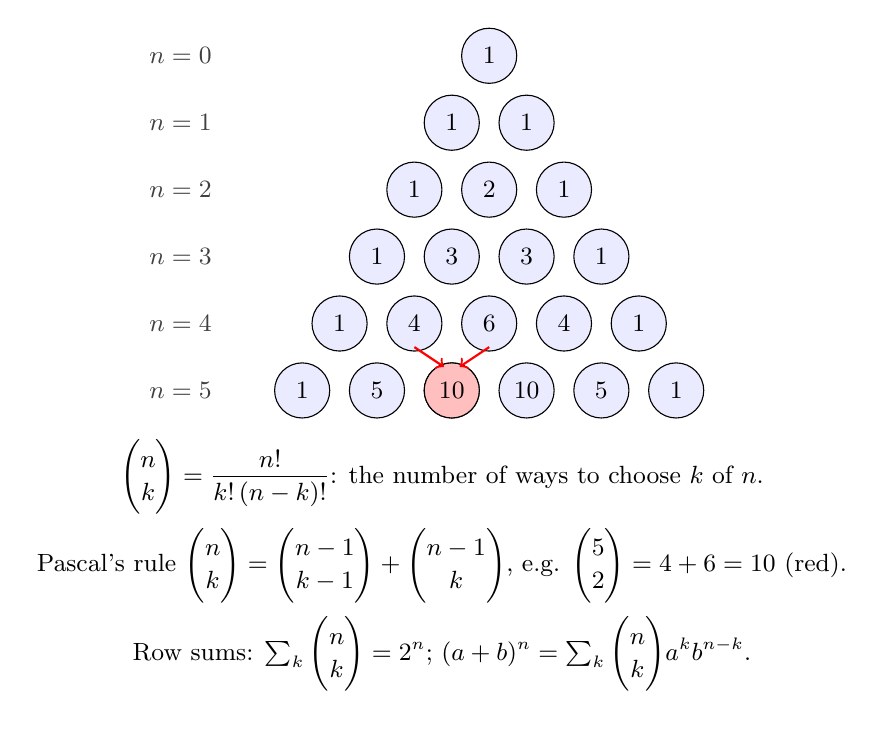
\begin{tikzpicture}[every node/.style={font=\small}]
	\foreach \n/\row in {0/{1}, 1/{1,1}, 2/{1,2,1}, 3/{1,3,3,1}, 4/{1,4,6,4,1}, 5/{1,5,10,10,5,1}} {
		\foreach \v [count=\k from 0] in \row {
			\node[draw, circle, fill=blue!8, minimum size=7mm, inner sep=0pt] at ({(\k-\n/2)*0.95},{-\n*0.85}) {$\v$};
		}
		\node[anchor=east, gray!50!black] at (-3.4,{-\n*0.85}) {$n=\n$};
	}
	\node[draw, circle, fill=red!25, minimum size=7mm, inner sep=0pt] at ({(2-2.5)*0.95},{-5*0.85}) {$10$};
	\draw[red, thick, ->] ({(1-2)*0.95},{-4*0.85-0.3}) -- ({(2-2.5)*0.95-0.1},{-5*0.85+0.3});
	\draw[red, thick, ->] ({(2-2)*0.95},{-4*0.85-0.3}) -- ({(2-2.5)*0.95+0.1},{-5*0.85+0.3});
	\node[anchor=north, align=center] at (-0.6,-4.75) {$\dbinom nk=\dfrac{n!}{k!\,(n-k)!}$: the number of ways to choose $k$ of $n$.\\[4pt] Pascal's rule $\dbinom nk=\dbinom{n-1}{k-1}+\dbinom{n-1}{k}$, e.g. $\dbinom52=4+6=10$ (red).\\[4pt] Row sums: $\sum_k\dbinom nk=2^n$; $(a+b)^n=\sum_k\dbinom nk a^kb^{n-k}$.};
\end{tikzpicture}
\end{document}
